\documentclass[a0paper,landscape,20pt]{extarticle}
\usepackage[margin=0.8in]{geometry}
\usepackage{multicol}
\usepackage{tikz}
\usepackage{pgfplots}
\usepackage{amsmath}
\usepackage{amssymb}
\usepackage{graphicx}
\usepackage{fancyhdr}
\usepackage{xcolor}
\usepackage{titlesec}
\usepackage{enumitem}

\usetikzlibrary{calc,shapes.geometric,arrows,positioning}
\pgfplotsset{compat=1.18}

% Define colors
\definecolor{darkblue}{RGB}{0,90,156}
\definecolor{mediumblue}{RGB}{0,123,191}
\definecolor{lightblue}{RGB}{173,216,230}
\definecolor{lightgray}{RGB}{245,245,245}

% Page setup
\pagestyle{empty}
\setlength{\columnsep}{2.5cm}
\setlength{\columnseprule}{2pt}
\def\columnseprulecolor{\color{mediumblue}}

% Title formatting
\titleformat{\section}{\huge\bfseries\color{darkblue}}{}{0em}{}[\vspace{0.4cm}\hrule height 3pt \vspace{0.6cm}]
\titleformat{\subsection}{\LARGE\bfseries\color{mediumblue}}{}{0em}{}[\vspace{0.3cm}]
\titleformat{\subsubsection}{\Large\bfseries\color{darkblue}}{}{0em}{}[\vspace{0.2cm}]

% Custom list formatting
\setlist[itemize]{leftmargin=*, topsep=0pt, itemsep=4pt}

\begin{document}

% Four column layout
\begin{multicols}{4}

%%%%%%%%%%%%%%%%%%%%%%%%%%%%%%%%%%%%%%%%%%%%%%%%%%%%%%%%%%%%%%%%%%%%%%%%%%%%%%
% COLUMN 1
%%%%%%%%%%%%%%%%%%%%%%%%%%%%%%%%%%%%%%%%%%%%%%%%%%%%%%%%%%%%%%%%%%%%%%%%%%%%%%

\section{Synthetic Aperture Radar}
\subsection{Principles, Applications, and Advanced Signal Processing}

\vspace{0.3cm}
\textbf{\Large Your Name$^1$, Co-Author Name$^2$, Senior Author Name$^1$}

\normalsize
$^1$Department of Electrical Engineering, Your University\\
$^2$Radar Systems Division, Research Institute\\
\texttt{\{email1, email2, email3\}@institution.edu}

\vspace{1.0cm}

\subsection{Introduction}

\textbf{Synthetic Aperture Radar (SAR)} is an advanced radar technique that creates high-resolution images of terrain and objects. Unlike conventional radar, SAR uses the motion of the radar antenna over a target region to provide finer spatial resolution than conventional beam-scanning radars.

\subsubsection{Key Advantages}
\begin{itemize}
  \item All-weather, day/night imaging capability
  \item High spatial resolution independent of range
  \item Penetration through clouds and vegetation
  \item Wide area coverage with fine detail
\end{itemize}

\subsubsection{Applications}
\begin{itemize}
  \item Earth observation and mapping
  \item Military surveillance and reconnaissance
  \item Environmental monitoring
  \item Disaster management and assessment
  \item Archaeological surveys
\end{itemize}

\subsection{SAR Geometry and Resolution}

\begin{center}
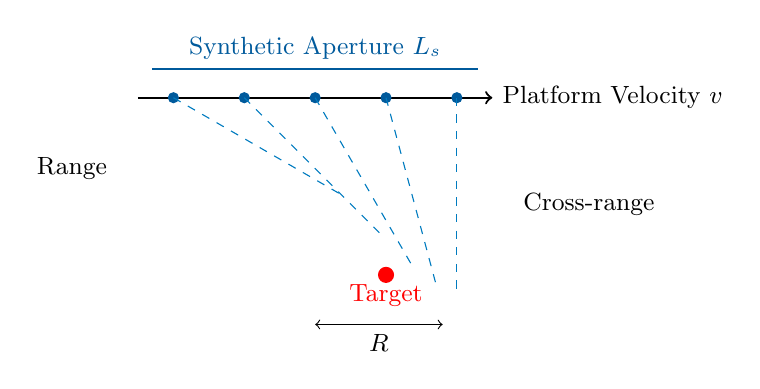
\begin{tikzpicture}[scale=0.9]
  % Draw platform trajectory
  \draw[thick, ->] (-2.5, 3) -- (2.5, 3) node[right] {\small Platform Velocity $v$};
  
  % Draw radar positions
  \foreach \x in {-2, -1, 0, 1, 2} {
    \filldraw[darkblue] (\x, 3) circle (2pt);
  }
  
  % Draw range lines
  \foreach \x/\angle in {-2/60, -1/45, 0/30, 1/15, 2/0} {
    \draw[dashed, mediumblue] (\x, 3) -- +(\angle+270:2.8);
  }
  
  % Draw target
  \filldraw[red] (1, 0.5) circle (3pt) node[below] {\small Target};
  
  % Draw synthetic aperture
  \draw[thick, darkblue] (-2.3, 3.4) -- (2.3, 3.4) node[midway, above] {\small Synthetic Aperture $L_s$};
  
  % Labels
  \node[left] at (-2.8, 2) {\small Range};
  \node[right] at (2.8, 1.5) {\small Cross-range};
  \draw[<->] (0, -0.2) -- (1.8, -0.2) node[midway, below] {\small $R$};
\end{tikzpicture}
\end{center}

\subsubsection{Resolution Equations}
\begin{align}
\rho_r &= \frac{c}{2B} \quad \text{(Range Resolution)}\\
\rho_a &= \frac{D}{2} \quad \text{(Azimuth Resolution)}
\end{align}

Where $c$ is speed of light, $B$ is bandwidth, and $D$ is antenna aperture.

%%%%%%%%%%%%%%%%%%%%%%%%%%%%%%%%%%%%%%%%%%%%%%%%%%%%%%%%%%%%%%%%%%%%%%%%%%%%%%
% COLUMN 2
%%%%%%%%%%%%%%%%%%%%%%%%%%%%%%%%%%%%%%%%%%%%%%%%%%%%%%%%%%%%%%%%%%%%%%%%%%%%%%

\subsection{SAR Signal Processing Chain}

\begin{center}
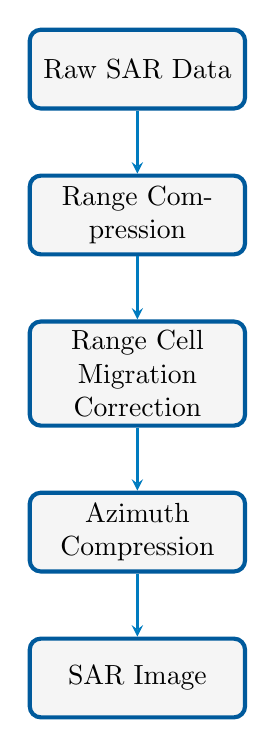
\begin{tikzpicture}[
  block/.style={rectangle, draw=darkblue, fill=lightgray, text width=2.5cm, text centered, rounded corners, minimum height=1cm, line width=1.5pt},
  arrow/.style={thick,->,>=stealth, color=mediumblue}
]
  \node[block] (raw) {Raw SAR Data};
  \node[block, below=0.8cm of raw] (range) {Range Compression};
  \node[block, below=0.8cm of range] (rcmc) {Range Cell Migration Correction};
  \node[block, below=0.8cm of rcmc] (azimuth) {Azimuth Compression};
  \node[block, below=0.8cm of azimuth] (image) {SAR Image};
  
  \draw[arrow] (raw) -- (range);
  \draw[arrow] (range) -- (rcmc);
  \draw[arrow] (rcmc) -- (azimuth);
  \draw[arrow] (azimuth) -- (image);
\end{tikzpicture}
\end{center}

\subsubsection{Range Compression}
Matched filtering of transmitted chirp signal:
$$s_c(t) = \text{IFFT}\{S(\omega) \cdot H^*(\omega)\}$$

\subsubsection{Azimuth Compression}
Focuses energy from synthetic aperture:
$$H_a(\omega) = \exp\left(j\frac{4\pi R_0}{\lambda}\sqrt{1-\left(\frac{\lambda\omega}{4\pi v}\right)^2}\right)$$

\subsubsection{Key Algorithms}
\begin{itemize}
  \item Range Doppler Algorithm (RDA)
  \item Chirp Scaling Algorithm (CSA)
  \item Frequency Scaling Algorithm (FSA)
  \item Back-projection Algorithm
\end{itemize}

\subsection{Range-Doppler Spectrum}

\begin{center}
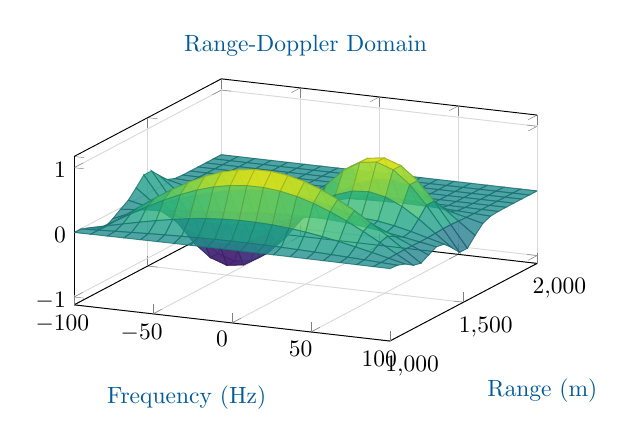
\begin{tikzpicture}[scale=0.85]
\begin{axis}[
  width=8.5cm,
  height=5.5cm,
  xlabel={Frequency (Hz)},
  ylabel={Range (m)},
  grid=major,
  grid style={gray!30},
  title style={color=darkblue},
  title={Range-Doppler Domain},
  colormap/viridis,
  xlabel style={color=darkblue},
  ylabel style={color=darkblue},
]
\addplot3[
  surf,
  samples=20,
  domain=-100:100,
  y domain=1000:2000,
  opacity=0.8,
] {sin(2*x)*exp(-(y-1500)^2/10000) + cos(x)*exp(-(y-1200)^2/8000)};
\end{axis}
\end{tikzpicture}
\end{center}

The Range-Doppler domain representation shows how targets appear as hyperbolic curves due to range migration effects during synthetic aperture formation.

%%%%%%%%%%%%%%%%%%%%%%%%%%%%%%%%%%%%%%%%%%%%%%%%%%%%%%%%%%%%%%%%%%%%%%%%%%%%%%
% COLUMN 3
%%%%%%%%%%%%%%%%%%%%%%%%%%%%%%%%%%%%%%%%%%%%%%%%%%%%%%%%%%%%%%%%%%%%%%%%%%%%%%

\subsection{SAR Imaging Modes}

\begin{center}
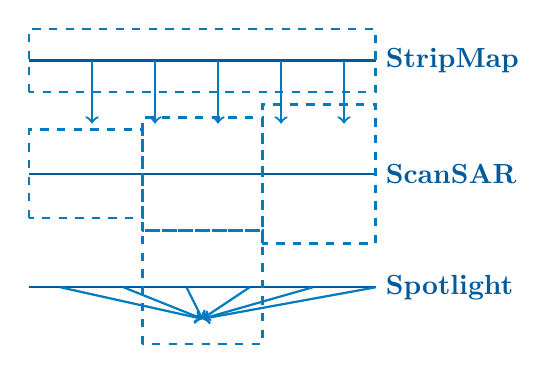
\begin{tikzpicture}[scale=0.8]
  % StripMap Mode
  \draw[thick, darkblue] (0,5) -- (5.5,5) node[right] {\textbf{StripMap}};
  \draw[dashed, mediumblue, line width=1pt] (0,4.5) rectangle (5.5,5.5);
  \foreach \x in {1,2,3,4,5} {
    \draw[->, thick, mediumblue] (\x,5) -- ++(0,-1);
  }
  
  % ScanSAR Mode  
  \draw[thick, darkblue] (0,3.2) -- (5.5,3.2) node[right] {\textbf{ScanSAR}};
  \draw[dashed, mediumblue, line width=1pt] (0,2.5) rectangle (1.8,3.9);
  \draw[dashed, mediumblue, line width=1pt] (1.8,2.3) rectangle (3.7,4.1);
  \draw[dashed, mediumblue, line width=1pt] (3.7,2.1) rectangle (5.5,4.3);
  
  % Spotlight Mode
  \draw[thick, darkblue] (0,1.4) -- (5.5,1.4) node[right] {\textbf{Spotlight}};
  \draw[dashed, mediumblue, line width=1pt] (1.8,0.5) rectangle (3.7,2.3);
  \foreach \x in {0.5,1.5,2.5,3.5,4.5,5.5} {
    \draw[->, thick, mediumblue] (\x,1.4) -- (2.75,0.9);
  }
\end{tikzpicture}
\end{center}

\subsubsection{Mode Characteristics}
\begin{itemize}
  \item \textbf{StripMap:} Wide swath, moderate resolution (1-10 m)
  \item \textbf{ScanSAR:} Very wide coverage, lower resolution  
  \item \textbf{Spotlight:} High resolution ($<$1 m), limited area
\end{itemize}

\subsection{Interferometric SAR (InSAR)}

\textbf{Principle:} Uses phase differences between SAR images to measure surface deformation and topography.

\begin{center}
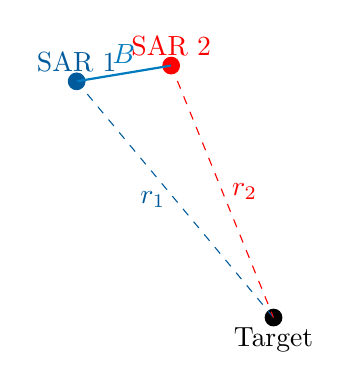
\begin{tikzpicture}[scale=1.0]
  % Two SAR positions
  \filldraw[darkblue] (0, 3) circle (3pt) node[above] {SAR 1};
  \filldraw[red] (1.2, 3.2) circle (3pt) node[above] {SAR 2};
  
  % Baseline
  \draw[thick, mediumblue] (0, 3) -- (1.2, 3.2) node[midway, above] {$B$};
  
  % Target
  \filldraw[black] (2.5, 0) circle (3pt) node[below] {Target};
  
  % Range vectors
  \draw[dashed, darkblue] (0, 3) -- (2.5, 0) node[midway, left] {$r_1$};
  \draw[dashed, red] (1.2, 3.2) -- (2.5, 0) node[midway, right] {$r_2$};
\end{tikzpicture}
\end{center}

$$\Delta\phi = \frac{4\pi}{\lambda}(r_2 - r_1)$$

\subsubsection{Applications}
\begin{itemize}
  \item Digital elevation models (DEM)
  \item Subsidence monitoring
  \item Earthquake deformation mapping
  \item Volcanic activity monitoring
\end{itemize}

\subsubsection{Height Accuracy}
$$\sigma_h = \frac{\lambda R \sin\theta}{4\pi B_\perp} \cdot \frac{\sigma_\phi}{\cos\theta}$$

%%%%%%%%%%%%%%%%%%%%%%%%%%%%%%%%%%%%%%%%%%%%%%%%%%%%%%%%%%%%%%%%%%%%%%%%%%%%%%
% COLUMN 4
%%%%%%%%%%%%%%%%%%%%%%%%%%%%%%%%%%%%%%%%%%%%%%%%%%%%%%%%%%%%%%%%%%%%%%%%%%%%%%

\subsection{Advanced Techniques}

\subsubsection{Compressive Sensing SAR}
Exploits sparsity in SAR images to reduce data requirements:
$\min_x \|x\|_1 \text{ subject to } \|Ax - b\|_2 < \epsilon$

\subsubsection{Machine Learning Integration}
\begin{itemize}
  \item Deep learning for image enhancement
  \item Automatic target recognition (ATR)
  \item Change detection algorithms
  \item Speckle reduction using CNNs
\end{itemize}

\subsubsection{Multi-Static SAR}
\begin{itemize}
  \item Distributed radar networks
  \item Improved resolution and coverage
  \item Reduced revisit times
  \item Enhanced target characterization
\end{itemize}

\subsection{Future Directions}

\subsubsection{Emerging Trends}
\begin{itemize}
  \item Miniaturized SAR systems (CubeSats)
  \item Real-time processing capabilities
  \item Multi-frequency and ultra-wideband SAR
  \item Integration with optical sensors
  \item AI-driven autonomous interpretation
\end{itemize}

\subsection{Key Takeaways}
\begin{itemize}
  \item SAR provides unique all-weather imaging capability
  \item Resolution is independent of range
  \item Multiple imaging modes serve different applications
  \item Advanced processing enables new capabilities
  \item Future developments focus on miniaturization and AI
\end{itemize}

\subsection{References}
\small
\setlength{\parindent}{0pt}
\setlength{\parskip}{0.3cm}

[1] Cumming, I. G., \& Wong, F. H. (2005). \textit{Digital processing of synthetic aperture radar data}. Artech house.

[2] Moreira, A., et al. (2013). A tutorial on synthetic aperture radar. \textit{IEEE Geoscience and Remote Sensing Magazine}, 1(1), 6-43.

[3] Bamler, R., \& Hartl, P. (1998). Synthetic aperture radar interferometry. \textit{Inverse problems}, 14(4), R1.

[4] Lee, J. S., \& Pottier, E. (2017). \textit{Polarimetric radar imaging: from basics to applications}. CRC press.

[5] Franceschetti, G., \& Lanari, R. (2018). \textit{Synthetic aperture radar processing}. CRC press.

[6] Rosen, P. A., et al. (2000). Synthetic aperture radar interferometry. \textit{Proceedings of the IEEE}, 88(3), 333-382.

\vspace{0.6cm}
\subsection{Contact Information}
\texttt{yourname@institution.edu}\\
\texttt{www.institution.edu/sar-lab}

\vspace{0.4cm}
\subsubsection{Acknowledgments}
\small
This work was supported by grants from [Funding Agency]. We thank our colleagues for valuable discussions and data sharing.

\end{multicols}

\end{document}

\end{document}